\documentclass[a4paper]{article}

\usepackage{INTERSPEECH2015}

\usepackage{graphicx}
\usepackage{amssymb,amsmath,bm}
\usepackage{textcomp}
\usepackage{multirow}

\def\vec#1{\ensuremath{\bm{{#1}}}}
\def\mat#1{\vec{#1}}


\sloppy
\ninept


\title{What Makes a Speaker Recognizable in TV Broadcast?\\
Going Beyond Speaker Identification Error Rate}


% \title{Speakers identification in broadcast TV: facilities and barriers}

%%%%%%%%%%%%%%%%%%%%%%%%%%%%%%%%%%%%%%%%%%%%%%%%%%%%%%%%%%%%%%%%%%%%%%%%%%
%% If multiple authors, uncomment and edit the lines shown below.       %%
%% Note that each line must be emphasized {\em } by itself.             %%
%% (by Stephen Martucci, author of spconf.sty).                         %%
%%%%%%%%%%%%%%%%%%%%%%%%%%%%%%%%%%%%%%%%%%%%%%%%%%%%%%%%%%%%%%%%%%%%%%%%%%
%\makeatletter
%\def\name#1{\gdef\@name{#1\\}}
%\makeatother
%\name{{\em Firstname1 Lastname1, Firstname2 Lastname2, Firstname3 Lastname3,}\\
%      {\em Firstname4 Lastname4, Firstname5 Lastname5, Firstname6 Lastname6,
%      Firstname7 Lastname7}}
%%%%%%%%%%%%%%% End of required multiple authors changes %%%%%%%%%%%%%%%%%

\makeatletter
\def\name#1{\gdef\@name{#1\\}}
\makeatother \name{{\em Delphine Charlet$^{1}$, Johann Poignant$^{2}$, Herv\'{e} Bredin$^{2}$, Corinne Fredouille$^{3}$, Sylvain Meignier$^{4}$}}

\address{$^1$ Orange Labs -- Lannion, France\\
         $^2$ LIMSI -- CNRS -- Orsay, France.\\
         $^3$ CERI/LIA -- University of Avignon -- Avignon, France\\
         $^4$ LIUM -- Universit\'e du Mans -- Le Mans, France \\
         {\small \tt delphine.charlet@orange.com}
}


\begin{document}

\maketitle

\begin{abstract}
\vspace*{-0.2cm}
Speaker identification approaches for TV broadcast are usually evaluated and compared based on global error rates derived from the overall duration of missed detection, false alarm and confusion.
Based on the analysis of the output of the systems submitted to the final round of the French evaluation campaign REPERE, this paper highlights the fact that these average metrics lead to the incorrect intuition that current state-of-the-art algorithms partially recognize all speakers. Setting aside incorrect diarization and adverse acoustic conditions, we show that their performance is in fact essentially bi-modal: in a given show, either all speech turns of a speaker are correctly identified or none of them are. We then proceed with trying to understand and explain this behavior, through perfomance prediction experiments. These experiments show that the most discriminant speaker characteristics are -- first -- their total speech duration in the current show and -- then only -- the amount of training data available to build their acoustic model.
\end{abstract}

\noindent{\bf Index Terms}: speaker recognition, error analysis, TV broadcast

\section{Introduction}
\label{sec:introduction}
For about five years, tremendous progress has been made in the speaker recognition field, especially for the speaker verification task in a phone environment. Supported by the evaluation campaigns organized by the National Institute of Standards and Technology (NIST)\cite{greenberg2013,greenberg2014}, this progress mainly relies on the development of the i-vector paradigm, which has definitely overtaken classical UBM/GMM \cite{bimbot2004}, or SVM \cite{wan2000} approaches. Inspired from the Joint Factor Analysis (JFA), which had already been applied with success in speaker detection, and which aims at estimating speaker and channel/session subspaces separately, the simpler and powerful i-vector-based modeling paradigm \cite{dehak2011} makes no distinction between both of subspaces thanks to a single total variability space, which covers both the speaker and session/channel variability. A large amount of studies has been dedicated to the enhancement of this paradigm, still in speaker verification, by coupling it with different channel compensation techniques\cite{dehak2011,bousquet2012,kanagasundaram2014}, or by investigating various scoring approaches, which directly embeds channel compensation\cite{kenny2010,dehak2011,garcia2011,jiang2012,bousquet2014}. 

When it comes to performance analysis, studies also mainly focus on speaker verification task.  In this framework, \cite{doddington98} have proposed a typology of speakers, using a menagerie lexicon, based on the observed properties of speakers to be more or less prone to miss detection or false alarm. Besides this typology, efforts have been made to identify the factors that may influence the performance of speaker verification. In \cite{kahn10}, the authors report dramatic variations of performance, when varying the choice of the training session, for a similar amount of training data; similar trend is observed, on a lesser extent, for testing data.  \cite{BESTanalysis} investigate a range of variabilities factors, divided in "intrinsic" variations and "extrinsic" variations where "intrinsic" refers to internal speaker variability issues such as speech style and vocal efforts, and "extrinsic" refers to sources of variability external to the speaker, such as microphone, channels, noise. Their experiments show, among others, the strong impact of the variation of the speech style.
In the field of speaker diarization, int the context of conference meetings, \cite{Huijbregts07theblame} have  tried to identify the main factors contributing to errors, and to quantify their impact, through a set of Oracle experiments. Their analysis showed that the speech analysis detector, followed by the overlapped speech, were the main causes of errors.

Very few recent studies  have concerned speaker identification in TV broadcast based on state-of-the-art speaker recognition systems. However, this context implies some non-trivial particularities such as the widely varying amount of training data and testing data per speaker, the properties of speech segments - duration, number, acoustic quality, etc - implied in the identification decision while processing an entire TV show, generally issued from a preliminary speaker diarization step, and finally the coverage of speaker dictionary used by the system and its direct impact on an open-set identification task (closer to real life applications). We propose in this paper to perform such performance analysis, on the 3 systems submitted to final round of the REPERE challenge \cite{KAHN--CBMI--2012}, which has enabled the development of multimodal identification systems. Here, the analysis is restricted to the so-called "mono-modal" systems, which only use speaker-voice to identify the speakers. We are interested in analyzing the performances obtained individually for each speaker, and the influence of some of their characteristics (for instance in terms of speech turns duration, etc ) on the obtained performance. In section \ref{sec:protocol}, the corpus, the systems and the evaluation measure are presented. In section \ref{sec:analysis}, the performance analysis is done, and the influence of some features on the performances are investigated in section \ref{sec:prediction} through a performance prediction paradigm.

\begin{table*}[t]
  \centering
  \begin{tabular}{|c|c|c|c|}
    \hline
    System          & PERCOL                                        & QCOMPERE                                        & SODA      \\
    \hline    
    Diarization     & two stage spk. diarization \cite{charlet2013} &  multi-stage spk. diarization \cite{Barras2006} & i-vector \cite{dupuy2014}         \\
                    & + overlapping speech detection                &                                                 &           \\
    \hline    
    SID             & ALIZE v3.0 toolkit \cite{larcher2013}         & Bob toolkit \cite{bob2012}                      & ALIZE v3.0 toolkit \cite{larcher2013}  \\
    \hline    
    feature         & 19 LFCC + $\delta$ coef,                      & 15 PLP-like cepstrum coef~\cite{Hermansky1990}  & 19 MFCC + $\delta$ coef,         \\
                    & + $\delta$ energy + 11 $\delta$$\delta$ coef  & 15 $\delta$ coef + $\delta$ energy              & + $\delta$ energy + 11 $\delta$$\delta$ coef  \\
    \hline    
    UBM             & gender independent                            & multi-lingual                                   & gender independent         \\
                    & 512 diagonal Gaussians                        & 256 diagonal Gaussians                          & 1024 diagonal Gaussians         \\
    \hline    
    i-vector        & 200 dim TVS estimated from                    & 400 dim TVS estimated from $39356$              & 300 dim TVS estimated from         \\
                    & 1200 spk. and 7500 sessions                   & speech segments (around $15$ seg./spk.)         & 680 spk. and 4150 sessions         \\
    \hline    
    Normalisation   & cepstral mean subtraction                     & Feature warping normalization                   & cepstral mean subtraction         \\
                    & and variance normalization                    & with a sliding window of $3$~s.~\cite{Pelecanos2001}.  &   and variance normalization        \\
    \hline    
    Training data   & 533 spk. id., min 30s, max 2mn30              & $706$ spk. id., min 30s                         & 680 spk. id., min 1mn , max 12 min         \\
    for i-vector    & (if higher, a set of i-vectors extracted)     & REPERE+ETAPE+French radio                       & REPERE+ETAPE+French radio+web         \\
                    & REPERE+ETAPE+French radio+web                 &                                                 &           \\            
    \hline    
    Decision        & CDS joined with Within-Class                  & PLDA                                            & PLDA         \\
                    & covariance normalization for                  & Eigen Factor Radial-based                       & Eigen Factor Radial-based       \\
                    & session/channel compensation                  & length normalization~\cite{bousquet2011}        &    length normalization      \\
    \hline                              
  \end{tabular}
  \caption{System comparison, TVS : total variability space, CDS: Cosine Distance Scoring}
  \label{tab:system}  
\end{table*}


\vspace*{-0.4cm}
\section{Experimental protocol}
\label{sec:protocol}

\subsection{Evaluation metrics}
\vspace*{-0.1cm}
We are interested in analysing speaker identification system performance, and particularly, the influence of some characteristics, in the training and the testing data. Thus, one speaker in a given show is considered as the unit of analysis, the so-called $SpkShow$. One speaker appearing in 2 different videos is considered as 2 distinct $SpkShow$. 

In this analysis, we adopt the point of view of the references: for each $SpkShow_i$ in the reference is computed a performance measure of the biometric system, defined as the F-measure of the detection of $SpkShow_i$. More precisely, defining $T^{ref}_i$ the total duration of $SpkShow_i$ in the reference, $T^{test}_i$ the total duration where $SpkShow_i$ is the system response and $T^{corr}_i$ the total duration of correct identification of $SpkShow_i$, Precision and Recall can be computed for each $SpkShow_i$:
\begin{itemize}
\item $Precision_i=\frac{T^{corr}_i}{T^{test}_i}$ ~~~~~~$Recall_i=\frac{T^{corr}_i}{T^{ref}_i}$
\item $Fm_i=\frac{2*Precision_i*Recall_i}{Precision_i+Recall_i}$
\end{itemize} 

Thus, $Fm_i=0$ means that $SpkShow_i$ was never correctly identified, whereas $Fm_i=1$ means that $SpkShow_i$ is perfectly identified, without miss detection nor false alarm.

\subsection{REPERE Corpus~\cite{Giraudel2012}}

The REPERE challenge~\cite{KAHN--CBMI--2012} is an evaluation campaign on multimodal person recognition (phase 1 took place in January 2013 and phase 2 in January 2014).  The systems evaluated in our experiments are the "mono-modal" systems (based only on voice-based speaker identification) submitted to phase2, on data set named \texttt{test2}, composed of 62 videos recorded from 8 different types of show (including news and talk shows) broadcasted from two French TV channels. 10 hours of speech are annotated, and contain 477 non-anonymous $SpkShow$, which have on average 6.2 speech turns each, for a mean duration of speech turn equal to 12.1s


%In table \ref{tab:test2} we detail the speaker repartition on the \texttt{test2} corpus.


%begin{table}[ht]
 % \centering
  %\begin{tabular}{|c|c|}
    %\hline
    %Part                                & \texttt{test2}    \\
    %\hline    
    %\# videos                           & 62                \\         
    %Annotated duration                  & 10 h.             \\
    %\hline      
    %$SpkShow$                           & 477               \\
    %\# speaker turns                    & 2981              \\
    %speech duration                     & 35929             \\
    %mean duration speech turns in s.    & 12.1 (15.32)      \\
    %\# speech turn per $SpkShow$        & 6.2 (10.7)        \\ 
   % \hline                              
  %\end{tabular}
  %\caption{Corpus size for the annotated part, number of $SpkShow$, speakers turns and speech duration for non-anonymous speakers. Mean duration of speech turns and number of speech turns par $SpkShow$, in parenthesis is the stantard deviation}
  %\label{tab:test2}  
%\end{table}


\subsection{Systems description}
\label{sec:systems}
brief description of the systems: training data, modelling, decision...
\subsection{PERCOL}

\subsection{QCOMPERE}

\subsection{SODA}







\section{Performance analysis}
\label{sec:analysis}


The table \ref{table-spkshow-perf} shows the average $Fm$ per $SpkShow$ for the different systems.
\begin{table*}[t]
\begin{center}
\begin{tabular}{r||c|c|c|c}
& Percol & Qcompere & Soda & Oracle \\\hline\hline
average $Fm$ & 0.361 & 0.381 & 0.351 & 0.462\\\hline
average $Fm$ for in dictionary speakers & 0.628 & 0.684 & 0.619 & 0.722\\\hline
\#$SpkShow$ out of dictionary & 200 & 209 & 204 & 172\\\hline
\#$SpkShow$ in dictionary & 277& 268 & 273 & 305\\\hline
\#$SpkShow$ in dictionary, with $Fm=0$ & 79 & 63 & 86 & 63\\\hline
\end{tabular}
\caption{Average system performances per $SpkShow$}
\label{table-spkshow-perf}
\end{center}
\end{table*}

From the table we can notice the important number of $SpkShow$ which are not in the dictionary of the system, about 40\% for each system. As they don't have any model, they obviously cannot be identified, leading to an average global $Fm$ rather poor. More interestingly, the number of $SpkShow$ which are actually in the dictionary and which are not recognised at all, is not negligeable: their represent between 23.5\% to 31.5\% of the in-dictionary $SpkShow$, according to the systems.


Figure~\ref{fig:FMeasureDistribution} plot the distribution of all the $SpkShow$ in the system dictionaries, according their performance $Fm$, for the different systems. Foreach $Spkshow$, the average performance and the maximal performance obtained across systems are computed, and the corresponding distribution are also plotted. We can see from this figure that the average performance (from 61.9\% to 68.9\% according to the systems) presented in table\ref{table-spkshow-perf} is not at all representative of the performances obtained foreach $SpkShow$: speakers are either not recognized or well recognized. Indeed, if we compute the average performance for $SpkShow$ which have $Fm \neq 0$, the average $Fm$ grows to 87.9\% for PERCOL, 89.5\% for QCompere and 90.3\% for SODA. 

% \begin{figure}[!h]
% \includegraphics[scale=0.6]{figures/PQS-mono-model.eps}
% \caption{$spkShow$ performance distribution, for each system}
% \label{PQS}
% \end{figure}

To evaluate the impact of the automatic speaker diarization, we also perform the speaker analysis performance, for systems applied on reference speaker diarization. Results for systems PERCOL is shown in Figure~\ref{fig:autoVSref}.  
The comparison of the speaker identification performance between using the reference or automatic speaker diarization, carried out on PERCOL and SODA systems, shows that 38 $SpkShow$ (over the 277 in-dictionary speakers) for PERCOL and 14 $SpkShow$ (over the 273 in-dictionary speakers) for SODA present a null f-measure ($Fm_i=0$) with the automatic speaker diarization and a f-measure above 0.9 (above 0.97 for PERCOL and 0.92 for SODA) with the reference one. For these particular $SpkShow$, the quality of the automatic speaker diarization is the main reason of the poor speaker identification performance since a fine-grained analysis of the speaker diarization outputs highlighted segment frontier errors, clustering confusion errors, or both of them. The purity of the clusters, on which the automatic speaker identification process is applied, is incriminated here. 
In addition, we considered the $SpkShow$ for which a null f-measure is obtained whatever the speaker diarization implied. This observation was made for 41 $SpkShow$ with PERCOL system and 72 with SODA system, 12 $SpkShow$ being common to both of them. Focusing on $SpkShow$ for which more than 10s are available for speaker identification in the speaker diarization reference, the amount of training data available per $SpkShow$  could not explain the poor performance observed (mean duration of 649,77s, minimum and maximum values of 34.19s and 5277.52s for PERCOL, mean duration of 613.3s, minimum and maximum values of 145.5s and 714.76s for SODA). 
To be independent of the intrinsic quality of the speaker identification systems, we focused our attention on the 12 common $SpkShow$ mentioned above by studying the reference segments involved in the speaker identification process. The analysis revealed that these segments were associated with very poor acoustic quality : a large amount of overlapped speech for 4 $SpkShow$ (from 20 to 90\% of overlapped speech according to  $SpkShow$), an entire interview made by phone for 1 $SpkShow$, poor sound quality with reverberation for 1 $SpkShow$, and large background noise (street, assembly background voices, applause, etc) or music for 8 of them.

\begin{figure}[t]
\centering
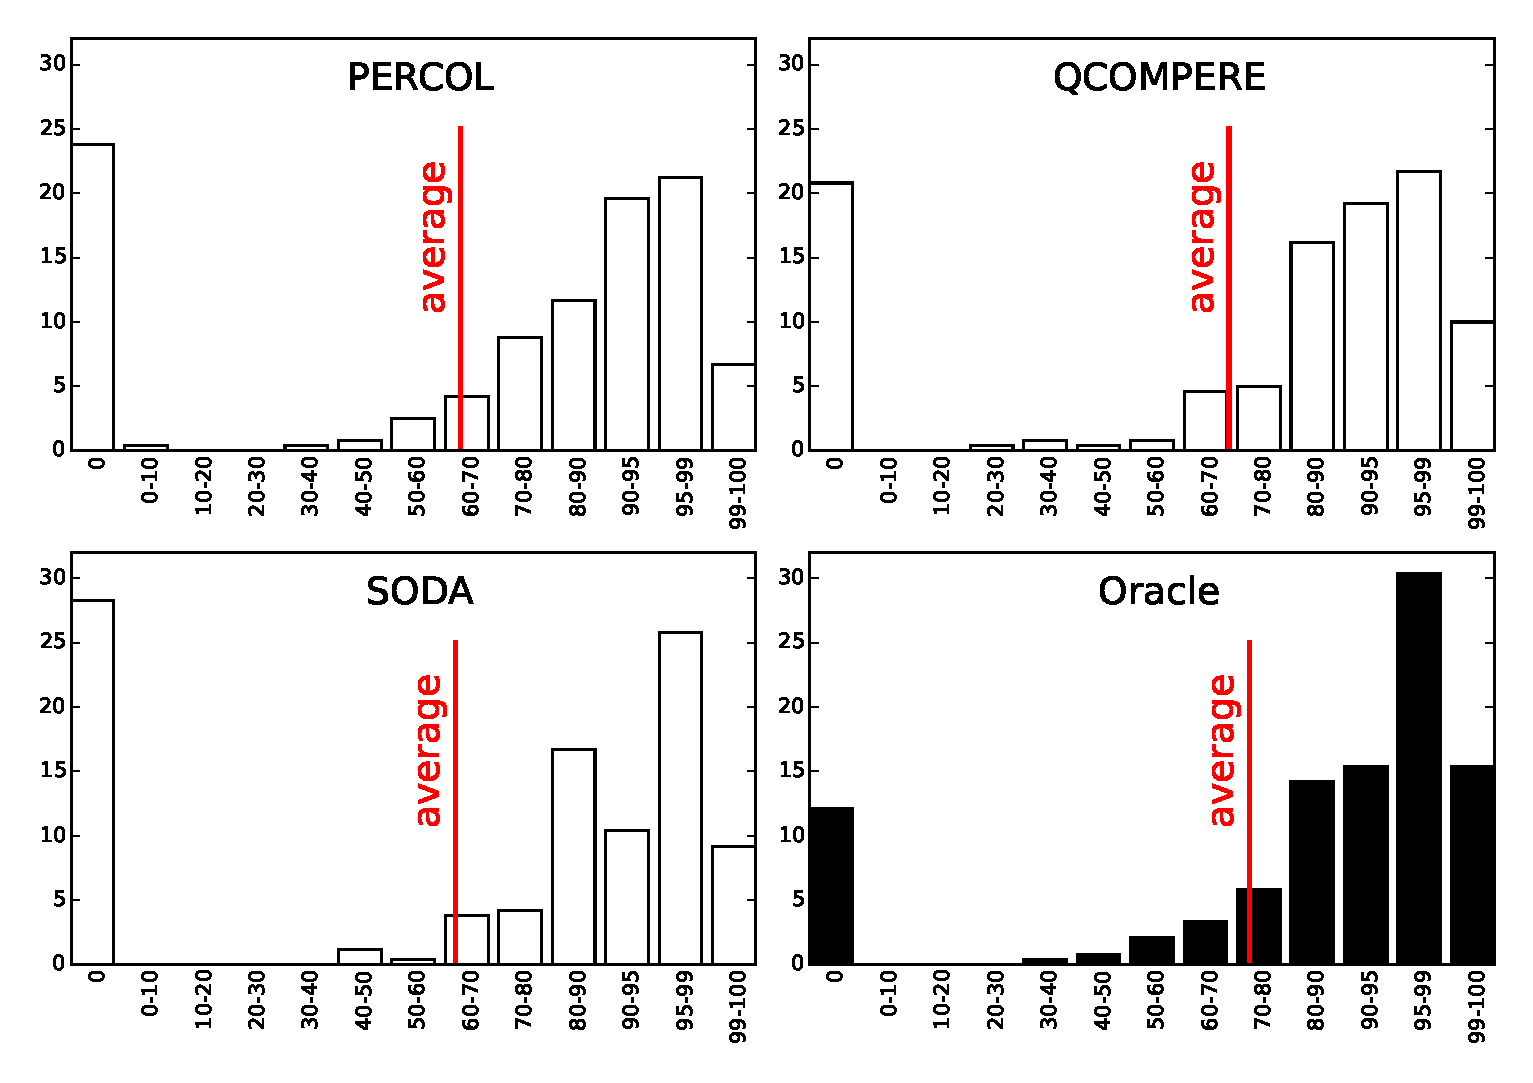
\includegraphics[width=\linewidth]{figures/bimodal.eps}
\caption{Distribution of $SpkShow$ according to system performance}
\label{fig:FMeasureDistribution}
\end{figure}


\begin{figure}[t]
\centering
\includegraphics[width=\linewidth]{figures/ref.eps}
\caption{Effect of segmentation errors on PERCOL.}
\label{fig:autoVSref}
\end{figure}



\section{Predicting speaker recognizability}
\label{sec:prediction}
We have seen in the previous section that speaker identification performance is essentially bi-modal: either a speaker is not recognized at all or it is very well recognized. This section aims at uncovering the speaker characteristics explaining why some speakers are recognized ($\checkmark$) and others are not ($\times$)? To answer this question, we first try to automatically classify the speakers into those two classes. In case we succeed, by analyzing the speaker characteristics contributing the most to this prediction, we should be able to identify the characteristics that facilitate or hamper the identification.

\subsection{$SpkShow$ characteristics}

Numerous characteristics could explain why a $SpkShow$ is recognized or not, including linguistic or prosodic characteristics or the background noise. In this paper, we only study two families of characteristics -- derived from the amount of training data used for speaker modeling, or related to the distribution of speech segments uttered by each speaker in the test set. 

The first set of characteristics includes the duration of training data available for each reference speaker (from the REPERE corpus, other corpora, or both) and the corresponding number of training sessions. For each $SpkShow$, these characteristics are obtained from the oracle system (\emph{i.e.} the system that performs the best for this particular $SpkShow$ among the three systems).

For each $SpkShow$, the second set of characteristics includes the number of speech turns, their total (or average) duration or the duration of the longest speech turn. It also includes characteristics related to the level of interactions of a $SpkShow$, such as the number and total duration of overlapped speech segments or the average pause duration before and after each speech turn of a $SpkShow$.

\subsection{Prediction of oracle performance}

Given a $SpkShow$ and its corresponding set of characteristics, we aim at predicting whether the oracle system is able to (at least partially) recognize $\checkmark$ it or not (at all) $\times$.  Focusing on oracle system enables to draw conclusions which are not specific of a given system.
As the corpus is limited (only 305 different $SpkShow$) and unbalanced (63 $\times$ vs. 242 $\checkmark$), we proceed using leave-one-out cross-validation and evaluate this classification experiment as two complementary detection tasks using precision, recall and F-measure.

Not all $SpkShow$ characteristics are meaningful features for this task, and some can even degrade the classification performance. 
Hence, feature selection is applied using the following heuristic.
Starting with the whole set of characteristics, each iteration removes the characteristic whose removal leads to the best performance.
The optimal subset of characteristics is selected as the one leading to the best overall performance.

As far as the classification algorithm is concerned, we chose to use a decision tree (rather than a more sophisticated black box classifier) as the analysis of its internal structure allows for easy interpretation of the results and the importance of each characteristic.
Table~\ref{tableresult} contains the experimental results. It shows that it is possible to predict, with pretty good performance, whether a $SpkShow$ will be recognized ($\checkmark$ $\text{F-measure} = 95.0\%$) or not ($\times$ $\text{F-measure} = 81.4\%$). 

\begin{table}[t]
\begin{center}
\begin{tabular}{|r|c|c|c|c|c|c|}
\hline
& \multicolumn{3}{c|}{All characteristics} & \multicolumn{3}{c|}{Optimal subset} \\
\hline
& P. & R. & F-measure & P. & R. & F-measure \\
\hline
$\checkmark$ & 94.5 & 93.4 & 94.0 & 95.6 & 94.6 & 95.0 \\
\hline
$\times$ & 75.8 & 79.0 & 77.4 & 80.0 & 82.7 & 81.4 \\
\hline
\end{tabular}
\caption{Prediction performance}
\label{tableresult}
\end{center}
\end{table}

\subsection{What makes a speaker recognizable?}

Now that we showed that it is possible to predict whether a $SpkShow$ is recognizable or not, this section aims at providing more insight into why this is the case.

Figure~\ref{fig:featureImportance} provides the distributions of \emph{feature importance} for the six characteristics selected in the optimal subset, computed over the 305 leave-one-out cross-validation rotations. 
Here, in the case of decision trees, feature importance is defined as the Gini coefficient and is related to the number of times a characteristic is used in the tree and how discriminant it is on average. More information on this metric can be found in~\cite{Breiman2001}
\begin{figure}[t]
\centering
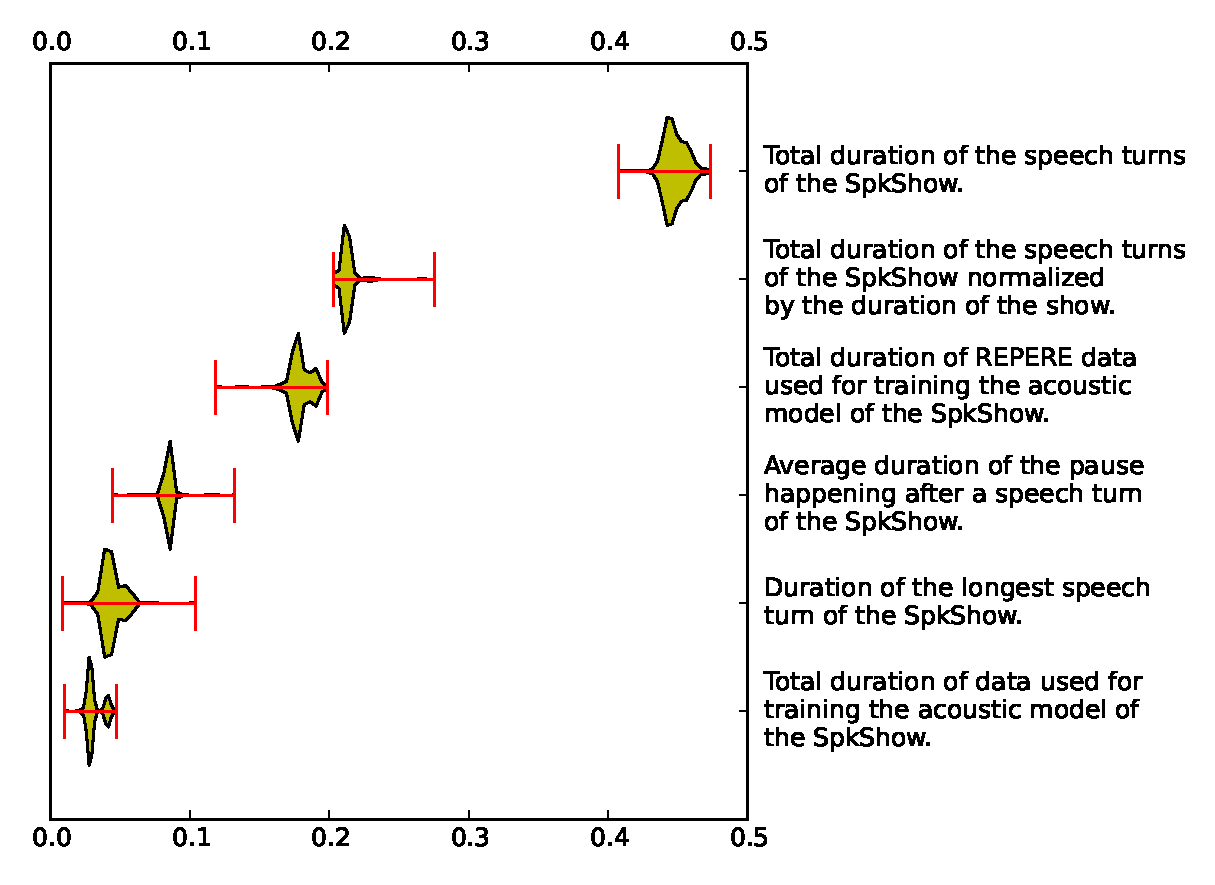
\includegraphics[width=\linewidth]{figures/violin.eps}
\caption{Distribution of feature importance.}
\label{fig:featureImportance}
\end{figure}

Interestingly, the two most important features are related to the duration of speech turns in the test set -- characteristics related to the amount of training data only appear at rank \#3 and \#6. 
The presence at rank \#4 of the characteristic defined as the average duration of the pause after each speech turn of a speaker is somewhat suprising. This could be explained by the fact that long pauses between two speech turns of two different speakers may ease the segmentation process (whose influence is discussed in Section~\ref{sec:analysis}) and therefore increase speaker recognizability.
Finally, Figure~\ref{fig:tree} is a graphical illustration of a decision tree (for sake of readability, the visualization is limited to depth 3) trained on the whole set of $SpkShow$ and based on the optimal subset of characteristics discussed in previous section. The boxes at the bottom represent the leaves of the decision tree. For each leaf, the label given by the tree is in the bottom right corner, and the box details the actual composition of $SpkShow$ classified in this leaf.
Noticeably, the rightmost leaf concentrates 195 out of the 242  $SpkShow$ which are recognized by the system ($\checkmark$), with only 2 simple rules about the minimal amount of testing data (10s) and training data in REPERE (30s).
%Talkative $SpkShow$ appear to be much easier to recognize than those with only a few short speech turns. When combined with lots of training data (see rightmost leaf), the former characteristic nearly always leads to good recognition (193 $\checkmark$ out of $305$ speakers!). 
\begin{figure}[t]
\centering
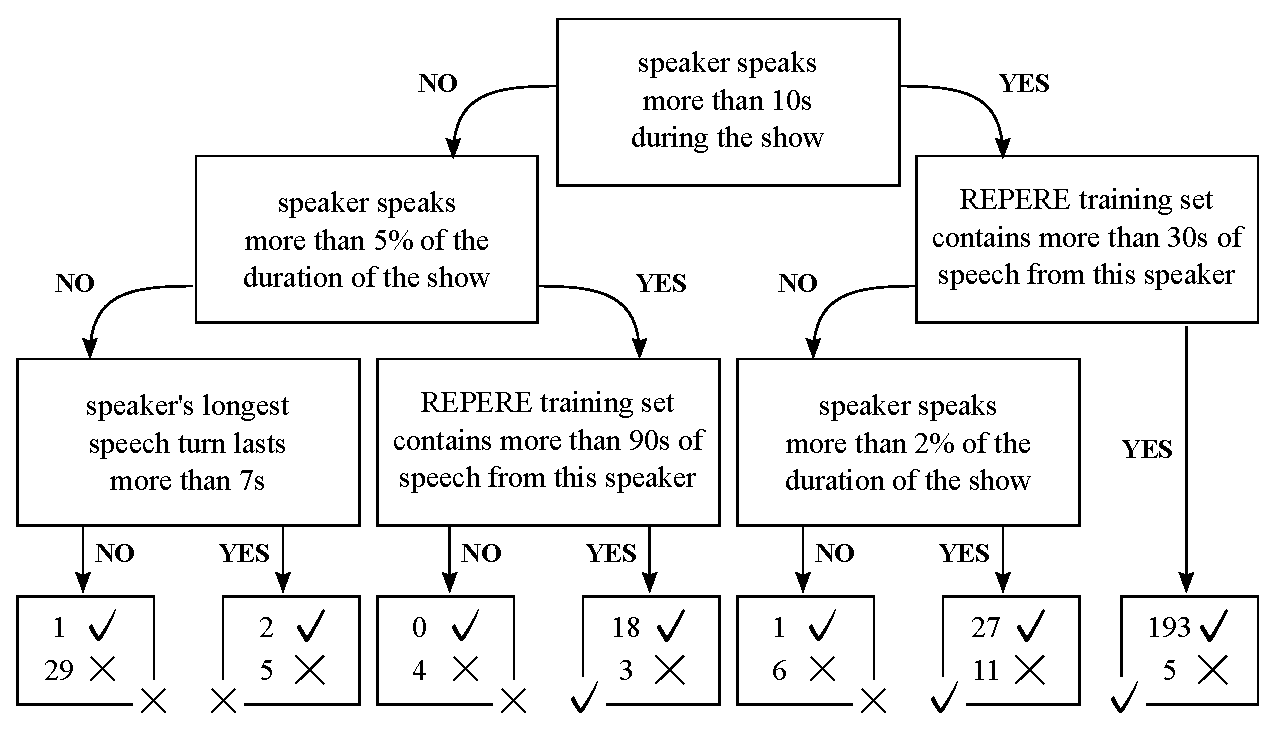
\includegraphics[width=\linewidth]{figures/tree.eps}
\caption{Not recognized ($\times$) vs. (partially) recognized ($\checkmark$)}
\label{fig:tree}
\end{figure}



% As anticipated, the amount of training data appears to be



\section{Conclusion}
\label{sec:conclusion}
\vspace*{-0.1cm}
In this paper, performance analysis has been done on 3 state-of-the-art i-vectors based speaker identification systems submitted on the REPERE challenge. It is shown that the performance distribution is essentiallty bi-modal: a speaker in a given show is either not recognized at all, or well recognized. A performance prediction paradigm has been developped, in order to predict if a speaker, with given characteristics in training and testing data will be recognized or not. This framework yields interesting prediction results  and enables to identify the characteristics which contribute the most to the correct recognition of the speakers.

%\section{Acknowledgements}

\newpage
\eightpt

\bibliographystyle{IEEEtran}
\bibliography{references}

\end{document}
